\documentclass[11pt,a4paper]{article}

% === Font & encoding (XeLaTeX) ===
\usepackage{fontspec}
\setmainfont{Latin Modern Roman}
\setsansfont{Latin Modern Sans}
\setmonofont{Latin Modern Mono}

% Korean font support via ucharclasses
\usepackage{ucharclasses}
\newfontfamily\koreanfont{Droid Sans Fallback}[Scale=0.95]
\setTransitionsForCJK{\koreanfont}{\setmainfont{Latin Modern Roman}}

% === Layout ===
\usepackage[margin=2cm,headheight=14pt]{geometry}
\usepackage{graphicx}
\usepackage{booktabs}
\usepackage{longtable}
\usepackage{float}
\usepackage{hyperref}
\usepackage{xcolor}
\usepackage{fancyhdr}
\usepackage{titlesec}
\usepackage{caption}
\usepackage{multirow}
\usepackage{enumitem}
\usepackage{array}
\usepackage{tabularx}
\usepackage{amssymb}
\usepackage[normalem]{ulem}

% === Header/Footer ===
\pagestyle{fancy}
\fancyhf{}
\rhead{V9 Cross-Model SAE Analysis}
\lhead{LLM Gambling Addiction}
\cfoot{\thepage}

% === Section styling ===
\titleformat{\section}{\Large\bfseries}{\thesection}{1em}{}
\titleformat{\subsection}{\large\bfseries}{\thesubsection}{1em}{}
\titleformat{\subsubsection}{\normalsize\bfseries}{\thesubsubsection}{1em}{}

% === Hyperlinks ===
\hypersetup{
    colorlinks=true,
    linkcolor=blue!60!black,
    citecolor=green!50!black,
    urlcolor=blue!70!black
}

% === Title ===
\title{\textbf{V9: Cross-Model, Cross-Domain Neural Basis of\\Risky Decision-Making in LLMs}\\[0.5em]
\large Internal Research Report (v9.5)\\[0.3em]
\normalsize ``Can Large Language Models Develop Gambling Addiction?''}
\author{Seungpil Lee, Donghyeon Shin, Yunjeong Lee, Sundong Kim\\
\small GIST (Gwangju Institute of Science and Technology)}
\date{March 19, 2026}

\begin{document}
\maketitle
\tableofcontents
\newpage

% ============================================================
% METADATA
% ============================================================
\noindent\textbf{Models}: Gemma-2-9B-IT (42L, 3584-dim, GemmaScope 131K) $|$ LLaMA-3.1-8B-Instruct (32L, 4096-dim, LlamaScope 32K)\\
\textbf{Paradigms}: Investment Choice (IC, 1600 games), Slot Machine (SM, 3200 games), Mystery Wheel (MW, 3200 games)\\
\textbf{Data}: Gemma: IC+SM+MW; LLaMA: IC+SM (MW pending)\\
\textbf{Pipeline}: StandardScaler $\rightarrow$ PCA(50) $\rightarrow$ LogReg(C=1.0, balanced) $|$ 5-fold StratifiedKFold

\medskip\noindent\textit{Data integrity: All numerical claims are traceable to computed JSON outputs.}

\bigskip\hrule\bigskip

% ============================================================
% CENTRAL QUESTION
% ============================================================
\section*{Central Question}
\addcontentsline{toc}{section}{Central Question}

\textbf{Do different models, across different gambling tasks, under different prompt conditions, share a common neural basis for bankruptcy --- the most extreme risk outcome?}

\begin{itemize}[nosep]
    \item \textbf{RQ1}: Do Gemma and LLaMA share common activation/feature patterns that predict bankruptcy?
    \item \textbf{RQ2}: Do activation patterns remain invariant when the domain (IC, SM, MW) changes?
    \item \textbf{RQ3}: Are neural representations consistent across prompt conditions (Fixed/Variable, G/M/W/P/R)?
\end{itemize}

% ============================================================
% EXECUTIVE SUMMARY
% ============================================================
\section*{Executive Summary}
\addcontentsline{toc}{section}{Executive Summary}

\textbf{RQ1 --- Universal BK Features Exist Across Architectures.}
600 of 3,584 Gemma L22 neurons (16.7\%) are sign-consistent universal BK predictors across three paradigms (FDR $p<0.01$). 744 SAE features across 7 layers show cross-domain consistency (L18+ binomial $p<5\times10^{-3}$). LLaMA achieves near-identical BK classification (AUC 0.974 vs Gemma 0.976 in SM). Factor decomposition confirms 65--71\% of SAE features encode BK independently of bet-type and paradigm (permutation $p=0.000$, null $\sim$1\%).

\medskip\textbf{RQ2 --- Strong Domain Invariance (Gemma), Selective Invariance (LLaMA).}
Gemma cross-domain transfer reaches AUC 0.87--0.93 (IC$\rightarrow$MW, SM$\rightarrow$MW; all $p=0.000$). A 3D shared BK subspace achieves AUC 0.86--0.97 despite near-orthogonal LR weight vectors. LLaMA IC$\rightarrow$SM transfer succeeds only at L25 (AUC 0.783), while SM$\rightarrow$IC is more stable (AUC 0.685 at L30). Hidden state transfer exceeds SAE transfer by 0.10--0.25 in most directions.

\medskip\textbf{RQ3 --- BK Representation Is Condition-Invariant, but Condition Effects Are Model-Dependent.}
LLaMA IC shows $\cos>0.81$ between Variable and Fixed BK directions across all layers ($n\ge65$ per group). Both models have $\sim$33--37\% shared BK neurons. G(Goal) dominates BK behaviorally in Gemma ($20.75\times$) but not LLaMA ($1.26\times$), yet both share the mechanism: G drives BK independently without modulating existing BK representations.

\bigskip\hrule\bigskip

% ============================================================
% 1. SETUP
% ============================================================
\section{Setup}

\subsection{Data \& Representations}

\begin{table}[H]
\centering
\caption{Dataset Overview}\label{tab:t1}
\footnotesize
\begin{tabular}{lccclll}
\toprule
Paradigm & Games & BK & BK\% & Bet Types & Constraints & Prompt Cond. \\
\midrule
IC (Gemma)  & 1,600 & 172   & 10.8\% & Fixed/Var & c10/c30/c50/c70 & BASE/G/M/GM \\
SM (Gemma)  & 3,200 & 87    & 2.7\%  & Fixed/Var & \$10 fixed      & 32 combos (G/M/W/P/R) \\
MW (Gemma)  & 3,200 & 54    & 1.7\%  & Fixed/Var & \$30 fixed      & 32 combos \\
IC (LLaMA)  & 1,600 & 142   & 8.9\%  & Fixed/Var & c10/c30/c50/c70 & BASE/G/M/GM \\
SM (LLaMA)  & 3,200 & 1,164 & 36.4\% & Fixed/Var & \$10 fixed      & 32 combos (G/M/H/W/P) \\
\bottomrule
\end{tabular}
\end{table}

\noindent\textbf{Hidden states}: Residual stream at each layer (Gemma: 3,584-dim $\times$ 42 layers; LLaMA: 4,096-dim $\times$ 32 layers).\\
\textbf{Decision Point (DP)}: Last decision time point. \textbf{Round 1 (R1)}: First round (\$100 equal balance).\\
\textbf{SAE}: GemmaScope 131K features/layer; LlamaScope 32K features/layer.

\subsection{V8 Limitations Addressed}

V8 (Gemma-only) left three weaknesses that V9 directly addresses:
\begin{enumerate}[nosep]
    \item \textbf{SAE cross-domain failure}: Only 1/131K features (\#101036) was sign-consistent at L22 top-50. V9: \textbf{744 features} across 7 layers (\S\ref{sec:sae744}).
    \item \textbf{Variable/Fixed ``dissociation''}: Artifact of comparing all games, not BK-only (\S\ref{sec:bkdir}).
    \item \textbf{Single model}: V9 adds LLaMA IC+SM (\S\ref{sec:crossmodel}, \S\ref{sec:llamatransfer}).
\end{enumerate}

\subsection{Cross-Model BK Rate Asymmetry}

\begin{table}[H]
\centering
\caption{BK Rate Asymmetry Between Models}\label{tab:t2}
\footnotesize
\begin{tabular}{lcccc}
\toprule
 & Gemma IC & LLaMA IC & Gemma SM & LLaMA SM \\
\midrule
Fixed BK rate    & \textbf{19.75\%} & 8.1\%  & --- & --- \\
Variable BK rate & 1.75\%  & \textbf{9.6\%}  & --- & --- \\
Overall BK rate  & 10.8\%  & 8.9\%  & 2.7\%  & \textbf{36.4\%} \\
Autonomy effect  & $-$18.0pp & $+$1.5pp & --- & --- \\
\bottomrule
\end{tabular}
\end{table}

\noindent Gemma IC: Fixed betting is 11$\times$ riskier than Variable. LLaMA IC: nearly equal. Gemma SM BK rate is 13$\times$ lower than LLaMA SM. These asymmetries complicate cross-model comparisons and must be considered when interpreting all subsequent analyses.

% ============================================================
% 2. RQ1
% ============================================================
\section{RQ1: Universal BK Features}

\subsection{600 Universal BK Neurons (Gemma L22, Hidden States)}

At L22, each of 3,584 neurons was tested for point-biserial correlation with BK outcome in each paradigm, with FDR correction (BH, $p<0.01$). Neurons significant in all three paradigms with consistent sign direction are ``Universal BK Neurons.''

\begin{table}[H]
\centering
\caption{Universal BK Neuron Summary (Gemma L22)}\label{tab:t3}
\footnotesize
\begin{tabular}{lcccc}
\toprule
 & IC & SM & MW & Cross-paradigm \\
\midrule
FDR-significant     & 2,528 (70.5\%) & 2,725 (76.0\%) & 2,314 (64.6\%) & --- \\
All-3-significant   & --- & --- & --- & 1,238 (34.5\%) \\
\textbf{Sign-consistent} & --- & --- & --- & \textbf{600 (16.7\%)} \\
BK-promoting        & --- & --- & --- & 302 \\
BK-inhibiting       & --- & --- & --- & 298 \\
\bottomrule
\end{tabular}
\end{table}

\begin{table}[H]
\centering
\caption{Top-5 Universal BK Neurons}\label{tab:t4}
\footnotesize
\begin{tabular}{ccccccl}
\toprule
Rank & Neuron & min$|r|$ & IC $r$ & SM $r$ & MW $r$ & Direction \\
\midrule
1 & \textbf{1763} & 0.217 & +0.305 & +0.248 & +0.217 & BK-promoting \\
2 & 371   & 0.203 & $-$0.223 & $-$0.203 & $-$0.209 & BK-inhibiting \\
3 & 2951  & 0.198 & $-$0.198 & $-$0.207 & $-$0.266 & BK-inhibiting \\
4 & 1755  & 0.190 & $-$0.210 & $-$0.198 & $-$0.190 & BK-inhibiting \\
5 & 864   & 0.182 & $-$0.267 & $-$0.182 & $-$0.182 & BK-inhibiting \\
\bottomrule
\end{tabular}
\end{table}

\noindent Neuron \#1763 is the strongest universal BK-promoting neuron (min$|r|=0.217$). Promoting (302) $\approx$ Inhibiting (298) at L22 --- balanced representation. This exactly reproduces V8's finding (600 neurons, \#1763 top).

\subsection{744 SAE Features with Cross-Domain Consistency (Gemma, 7 Layers)}\label{sec:sae744}

V8 examined only L22 top-50 features (0.038\% of 131K). V9 tests 7 informative layers (L10, 12, 18, 22, 26, 30, 33) using all active features. A feature is ``sign-consistent'' if its Cohen's $d$ has the same sign across IC, SM, and MW, with geometric mean $|d| \ge 0.2$ for ``strong'' features.

\begin{table}[H]
\centering
\caption{Gemma Multi-Layer SAE Cross-Domain Consistency}\label{tab:t5}
\footnotesize
\begin{tabular}{lcccc}
\toprule
Layer & Active & Sign-consistent & Strong ($d\ge0.2$) & \% consistent \\
\midrule
L10 & 92  & 30  & 23  & 32.6\% \\
L12 & 112 & 35  & 31  & 31.2\% \\
L18 & 170 & 58  & 52  & 34.1\% \\
L22 & 281 & 109 & 95  & 38.8\% \\
L26 & 303 & 133 & 119 & 43.9\% \\
L30 & 415 & 188 & 173 & 45.3\% \\
L33 & 456 & 191 & 172 & 41.9\% \\
\midrule
\textbf{Total} & --- & \textbf{744} & \textbf{665} & --- \\
\bottomrule
\end{tabular}
\end{table}

\noindent V8 baseline: 1 feature $\rightarrow$ V9: 744 features (665 strong).

\begin{table}[H]
\centering
\caption{Binomial Test Against Chance (3-paradigm chance = 25\%)}\label{tab:t6}
\footnotesize
\begin{tabular}{lccc}
\toprule
Layer & Observed \% & Binomial $p$ (vs 25\%) & Significant? \\
\midrule
L10 & 32.6\% & 6.2e-02 & NS \\
L12 & 31.2\% & 8.0e-02 & NS \\
L18 & 34.1\% & 4.9e-03 & ** \\
L22 & 38.8\% & 2.4e-07 & *** \\
L26 & 43.9\% & 6.5e-13 & *** \\
L30 & 45.3\% & 2.5e-19 & *** \\
L33 & 41.9\% & 2.5e-15 & *** \\
\bottomrule
\end{tabular}
\end{table}

\begin{figure}[H]
\centering
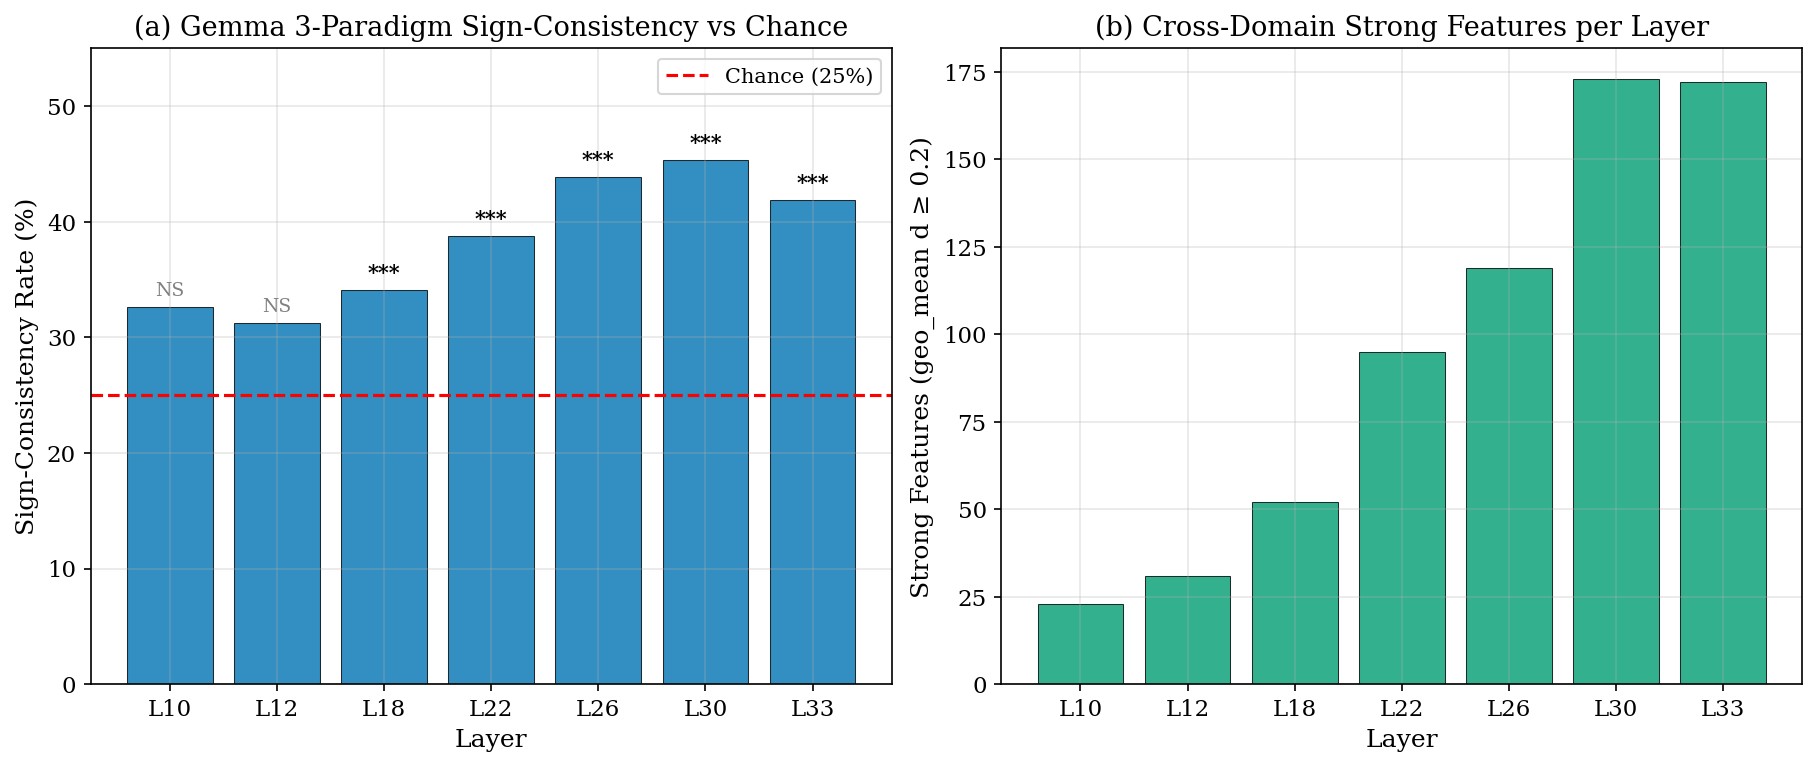
\includegraphics[width=\textwidth]{figures/fig1_crossdomain_consistency.png}
\caption{Gemma 3-paradigm sign-consistency with binomial test. (a) L10--L12 do not exceed chance (25\%, red dashed). L18+ far exceeds chance (***). (b) Strong features peak at L30 (173). Deep-layer cross-domain signal is robust; shallow-layer apparent consistency is noise.}
\label{fig:f1}
\end{figure}

\subsection{Cross-Model Comparison (Gemma vs LLaMA)}\label{sec:crossmodel}

\begin{table}[H]
\centering
\caption{BK Classification AUC (DP, SAE $\rightarrow$ PCA $\rightarrow$ LogReg)}\label{tab:t7}
\footnotesize
\begin{tabular}{lcc}
\toprule
Paradigm & Gemma-2-9B & LLaMA-3.1-8B \\
\midrule
SM best AUC & \textbf{0.976} (L20) & \textbf{0.974} (L8) \\
IC best AUC & \textbf{0.960} (L30) & \textbf{0.954} (L12) \\
\bottomrule
\end{tabular}
\end{table}

\begin{table}[H]
\centering
\caption{LLaMA SM AUC Across Layers}\label{tab:t8}
\footnotesize
\begin{tabular}{lccc}
\toprule
Layer & AUC & n\_features & n\_BK \\
\midrule
L0  & 0.970 & 157   & 1,164 \\
L4  & 0.971 & 750   & 1,164 \\
\textbf{L8}  & \textbf{0.974} & 818   & 1,164 \\
L12 & 0.973 & 854   & 1,164 \\
L15 & 0.970 & 962   & 1,164 \\
L20 & 0.963 & 1,028 & 1,164 \\
L25 & 0.961 & 1,182 & 1,164 \\
L30 & 0.959 & 1,368 & 1,164 \\
\bottomrule
\end{tabular}
\end{table}

\begin{table}[H]
\centering
\caption{SAE BK-Differential Features (SM, $d\ge0.3$)}\label{tab:t9}
\footnotesize
\begin{tabular}{lcccc}
\toprule
Layer & Gemma SM & Gemma BK+/BK$-$ & LLaMA SM & LLaMA BK+/BK$-$ \\
\midrule
L10 & 71  & 42 / 29  & 322 & 160 / 162 \\
L22 & 286 & 125 / 161 & 251 & 135 / 116 \\
L30 & 452 & 165 / 287 & 381 & 160 / 221 \\
\bottomrule
\end{tabular}
\end{table}

\begin{table}[H]
\centering
\caption{R1 Within-Bet-Type Classification}\label{tab:t10}
\footnotesize
\begin{tabular}{lcc}
\toprule
Paradigm / Bet type & AUC (Gemma IC, L22) & AUC (LLaMA IC, L10) \\
\midrule
Fixed    & 0.755 (n=800, BK=158) & 0.786 (n=800, BK=65) \\
Variable & 0.665 (n=800, BK=14)  & 0.798 (n=800, BK=77) \\
SM Variable & 0.801 (n=1600, BK=87) & --- \\
\bottomrule
\end{tabular}
\end{table}

\begin{figure}[H]
\centering
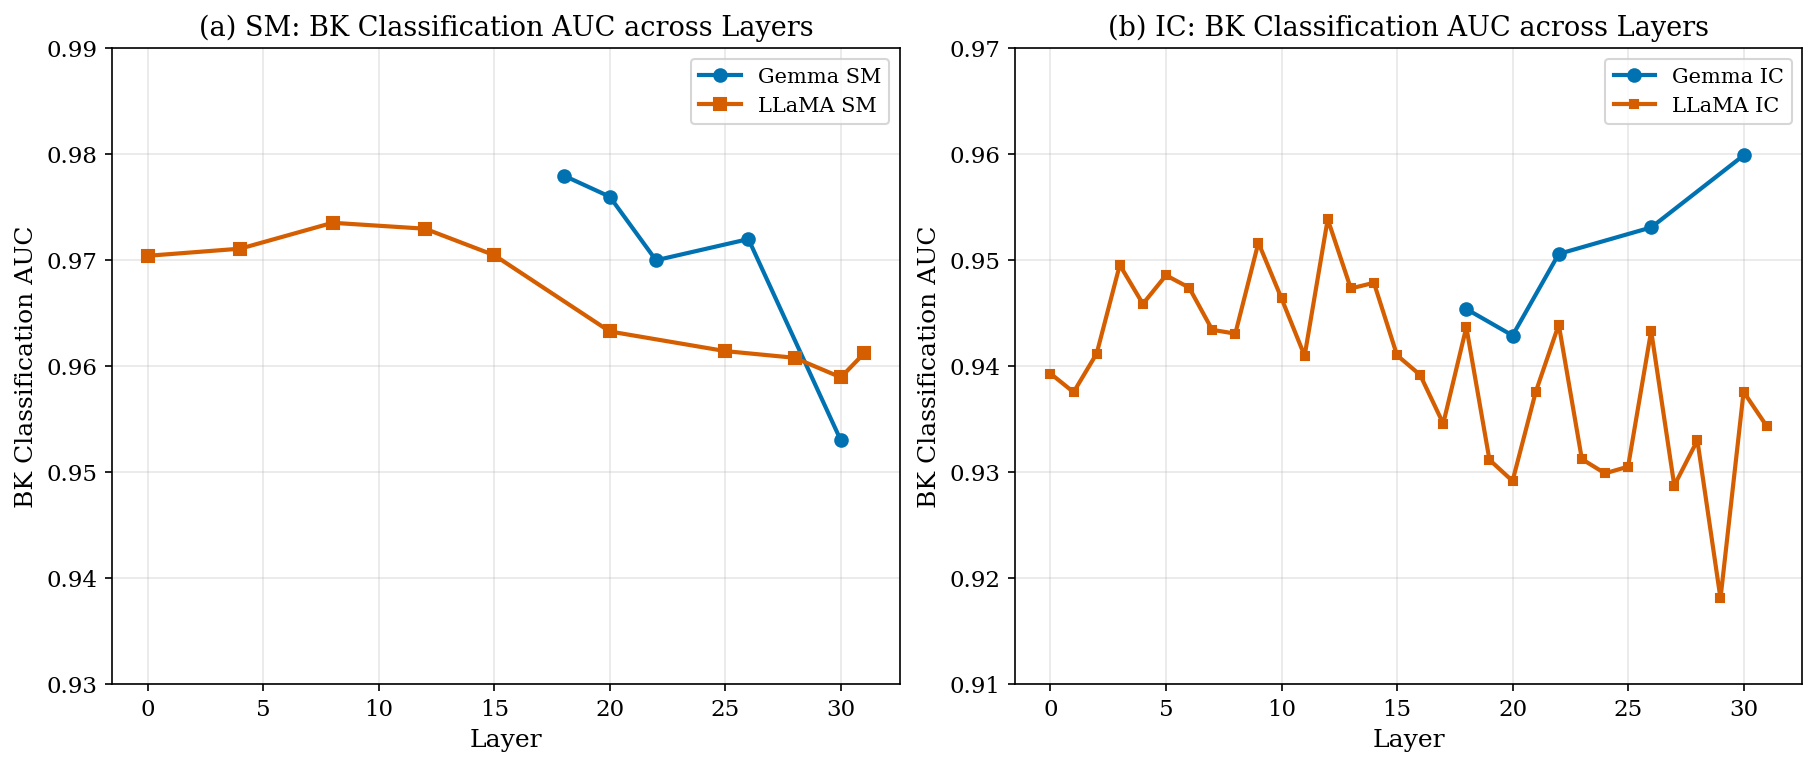
\includegraphics[width=\textwidth]{figures/fig6_classification_auc.png}
\caption{BK classification AUC across layers --- cross-model comparison. (a) SM: both models AUC $> 0.95$ (Gemma peaks L18--20, LLaMA peaks L8). (b) IC: Gemma peaks L30 (0.960), LLaMA peaks L12 (0.954). Encoding depth differs but performance is near-identical.}
\label{fig:f2}
\end{figure}

\subsection{RQ1 Synthesis}

Cross-model commonalities:
\begin{enumerate}[nosep]
    \item \textbf{Near-identical BK prediction}: 0.976 vs 0.974 (SM) --- architecture-invariant information content.
    \item \textbf{BK-inhibiting dominance at L30}: Both models (all $p < 0.001$). Not at L22 (LLaMA SM: $p=0.897$).
    \item \textbf{Encoding depth differs}: Gemma peaks mid-deep (L20), LLaMA peaks early (L8). Where BK is encoded is architecture-dependent; that it exists is not.
    \item \textbf{R1 early prediction}: AUC 0.665--0.801 from Round 1 --- BK signals exist from game start.
    \item \textbf{Factor decomposition}: 65.2\% (Gemma) and 69.5\% (LLaMA) of SAE features encode BK independently (perm $p=0.000$, null $\sim$1\%). BK representation has an independent axis in both architectures.
\end{enumerate}

% ============================================================
% 3. RQ2
% ============================================================
\section{RQ2: Domain Invariance}

\subsection{Hidden State Cross-Domain Transfer (Gemma L22)}

Gemma L22 DP hidden states: PCA(50) $\rightarrow$ LogReg(balanced) $\rightarrow$ cross-paradigm AUC. 200-permutation test for significance. Note: Table~\ref{tab:t11} compares HS vs SAE at the \emph{same layer} (L22), while Table~\ref{tab:t12} reports the \emph{best layer} per direction.

\begin{table}[H]
\centering
\caption{Hidden State vs SAE Transfer (Gemma L22, same-layer comparison)}\label{tab:t11}
\footnotesize
\begin{tabular}{lcccc}
\toprule
Transfer & Hidden AUC & SAE AUC & $\Delta$ (HS$-$SAE) & HS perm\_$p$ \\
\midrule
IC $\rightarrow$ SM & \textbf{0.746} & 0.499 (NS) & +0.247 & 0.000 \\
IC $\rightarrow$ MW & \textbf{0.826} & 0.876 & $-$0.050 & 0.000 \\
SM $\rightarrow$ MW & \textbf{0.920} & 0.819 & +0.101 & 0.000 \\
\bottomrule
\end{tabular}
\end{table}

\noindent Hidden state transfer exceeds SAE transfer in IC$\rightarrow$SM (+0.247) and SM$\rightarrow$MW (+0.101). In IC$\rightarrow$MW, SAE slightly outperforms hidden states. V8's ``hidden $>$ SAE'' claim is confirmed for 2 of 3 directions. BK signal is distributed --- SAE sparsification loses coherence in IC$\rightarrow$SM.

\subsection{SAE Cross-Domain Transfer with Permutation Test (Gemma)}

For each (train, test) paradigm pair at layers [18, 22, 26, 30]: common active features ($\ge$1\% rate in both) $\rightarrow$ StandardScaler $\rightarrow$ PCA(50) $\rightarrow$ LogReg $\rightarrow$ AUC. 200-permutation null.

\begin{table}[H]
\centering
\caption{Best SAE Transfer AUC Per Direction (Gemma, layer-optimal)}\label{tab:t12}
\footnotesize
\begin{tabular}{lcccc}
\toprule
Transfer & Best Layer & AUC & perm\_$p$ & Null mean \\
\midrule
IC $\rightarrow$ SM & L26 & \textbf{0.913} & 0.000 & 0.498 \\
IC $\rightarrow$ MW & L18 & \textbf{0.932} & 0.000 & 0.504 \\
SM $\rightarrow$ MW & L30 & \textbf{0.867} & 0.000 & 0.504 \\
SM $\rightarrow$ IC & L30 & 0.646 & 0.000 & 0.500 \\
MW $\rightarrow$ IC & L22 & 0.853 & 0.000 & 0.500 \\
\bottomrule
\end{tabular}
\end{table}

\begin{table}[H]
\centering
\caption{Layer-by-Layer SAE Transfer (Gemma, Key Directions)}\label{tab:t13}
\footnotesize
\begin{tabular}{lcccccc}
\toprule
Layer & IC$\rightarrow$SM & $p$ & IC$\rightarrow$MW & $p$ & SM$\rightarrow$MW & $p$ \\
\midrule
L18 & 0.719 & 0.000 & 0.932 & 0.000 & 0.789 & 0.000 \\
L22 & 0.499 & 0.485 (NS) & 0.876 & 0.000 & 0.819 & 0.000 \\
L26 & \textbf{0.913} & 0.000 & 0.883 & 0.000 & 0.866 & 0.000 \\
L30 & 0.529 & 0.175 (NS) & 0.767 & 0.000 & 0.867 & 0.000 \\
\bottomrule
\end{tabular}
\end{table}

\noindent IC$\rightarrow$MW and SM$\rightarrow$MW transfer work consistently across all layers. IC$\rightarrow$SM transfer is layer-dependent: L26 succeeds (0.913) but L22 fails (0.499 NS). This indicates IC and SM representations align only at specific layers.

\begin{figure}[H]
\centering
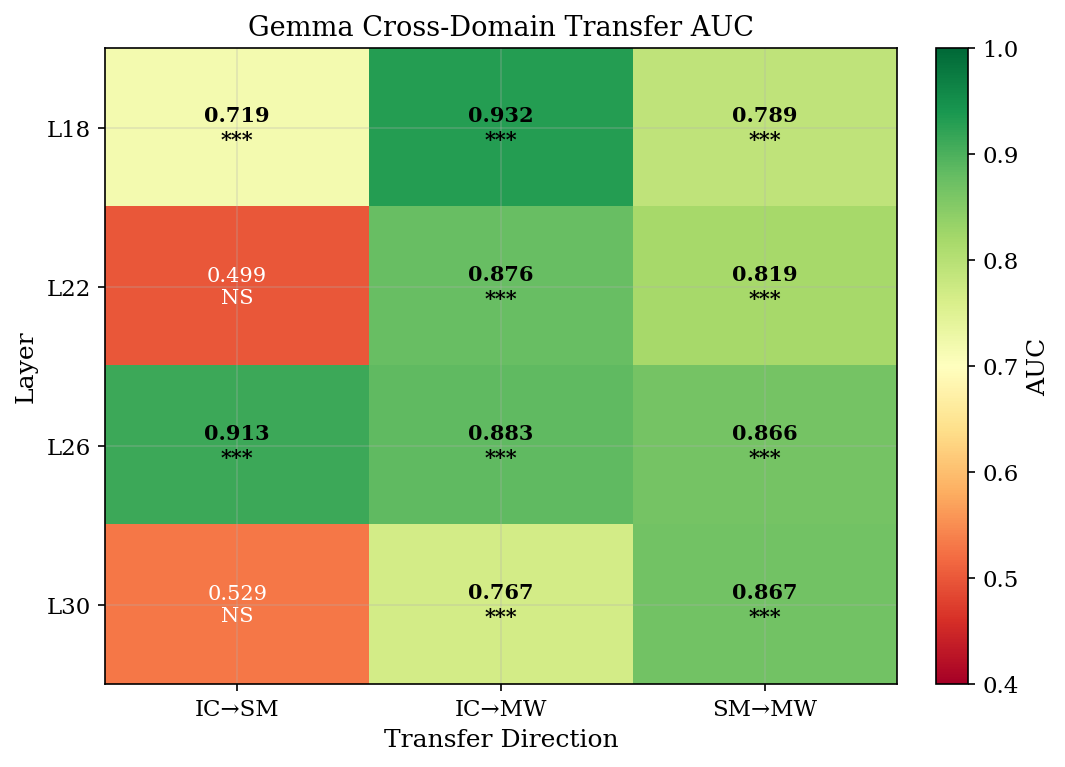
\includegraphics[width=\textwidth]{figures/fig4_transfer_heatmap.png}
\caption{Gemma cross-domain transfer AUC heatmap. IC$\rightarrow$MW (0.77--0.93) and SM$\rightarrow$MW (0.79--0.87) are significant at all layers. IC$\rightarrow$SM is layer-dependent (L26: 0.913***, L22: 0.499 NS). Red cells indicate transfer failure.}
\label{fig:f3}
\end{figure}

\subsection{3D Shared BK Subspace (Gemma L22)}

PCA of 3 paradigm-specific LR weight vectors yields a 3D BK subspace:

\begin{table}[H]
\centering
\caption{3D Shared Subspace Performance}\label{tab:t14}
\footnotesize
\begin{tabular}{lcc}
\toprule
Paradigm & 3D Subspace AUC & Full-dim AUC (50-PC) \\
\midrule
IC & 0.862 $\pm$ 0.029 & $\sim$0.95+ \\
SM & 0.899 $\pm$ 0.034 & $\sim$0.97+ \\
MW & 0.970 $\pm$ 0.016 & $\sim$0.97+ \\
\bottomrule
\end{tabular}
\end{table}

\noindent LR weight vector cosines: IC--SM=0.042, IC--MW=$-$0.026, SM--MW=$-$0.026 (near-orthogonal). Despite orthogonal weight vectors, the 3D subspace achieves AUC 0.86--0.97 --- BK signal is distributed across a subspace, not a single direction. Consistent with V8 (0.91--0.94).

\subsection{Factor Decomposition (Gemma 3-paradigm, LLaMA 2-paradigm)}

Per-feature OLS regression: \texttt{feature $\sim$ outcome + bet\_type + paradigm}. Features where outcome is significant ($p<0.01$) after controlling bet\_type and paradigm encode BK independently.

\begin{table}[H]
\centering
\caption{Factor Decomposition: Outcome-Significant Features}\label{tab:t15}
\footnotesize
\begin{tabular}{lcc}
\toprule
Factor & Gemma (581 feat., IC+SM+MW) & LLaMA (1,418 feat., IC+SM) \\
\midrule
\textbf{Outcome} (BK) & \textbf{65.2\%} (379) & \textbf{69.5\%} (985) \\
Bet-type            & 92.3\% & 81.4\% \\
Paradigm            & 99.8\% & 96.2\% \\
\bottomrule
\end{tabular}
\end{table}

\noindent Permutation validation (selfcritique rerun): null outcome-significant $\approx$1\% $\rightarrow$ observed 65--71\% yields perm\_$p$=0.000. BK representation's independent existence is statistically established in both architectures.

\begin{figure}[H]
\centering
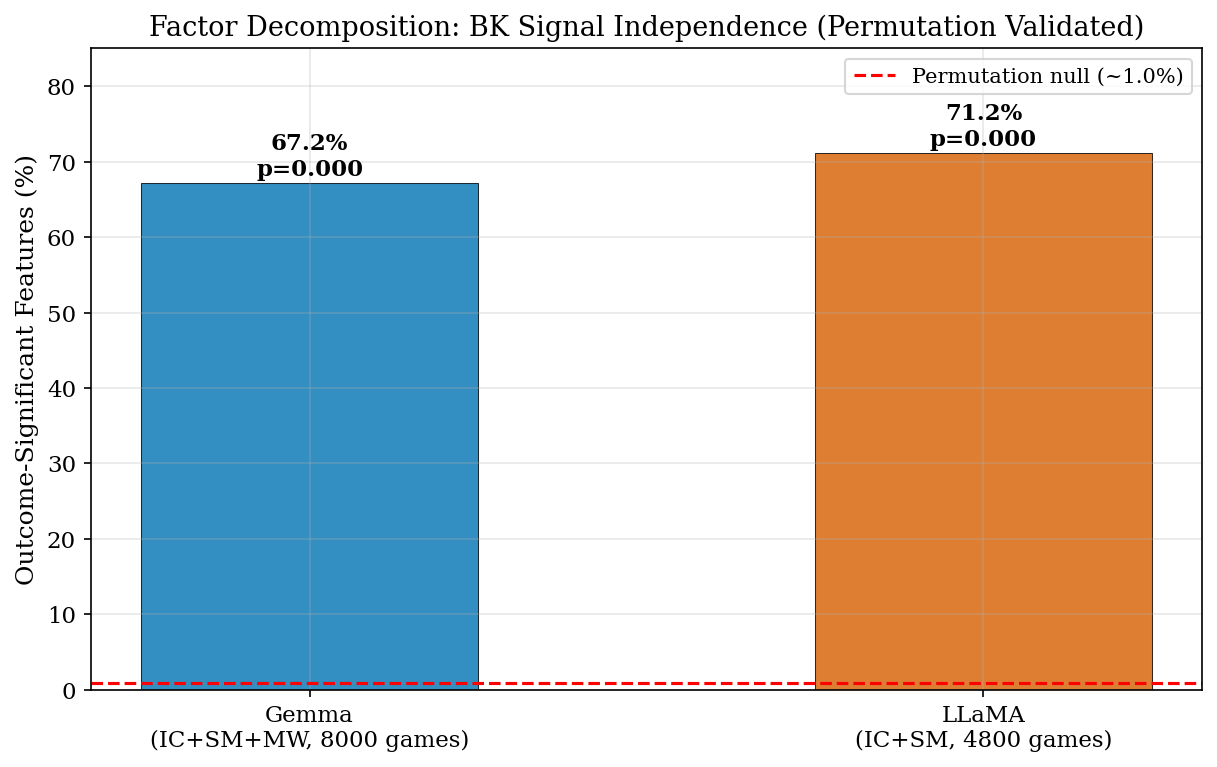
\includegraphics[width=\textwidth]{figures/fig3_factor_decomposition.png}
\caption{Factor decomposition with permutation test. Both models: 65--71\% outcome-significant (blue/orange), exceeding null ($\sim$1\%, dashed) by $60\times$+. Perm $p=0.000$. BK representation independence is architecture-invariant.}
\label{fig:f4}
\end{figure}

\subsection{LLaMA Cross-Domain Transfer (IC $\leftrightarrow$ SM)}\label{sec:llamatransfer}

LLaMA IC ($n$=1,600, BK=142) $\leftrightarrow$ SM ($n$=3,200, BK=1,164). SAE features $\rightarrow$ PCA(50) $\rightarrow$ LogReg $\rightarrow$ AUC. 200-permutation test.

\begin{table}[H]
\centering
\caption{LLaMA IC$\leftrightarrow$SM Transfer}\label{tab:t16}
\footnotesize
\begin{tabular}{llccc}
\toprule
Transfer & Layer & AUC & perm\_$p$ & Null mean \\
\midrule
IC $\rightarrow$ SM & L25 & \textbf{0.783} & 0.000 & 0.500 \\
IC $\rightarrow$ SM & L15 & 0.522 & 0.020 & 0.501 \\
IC $\rightarrow$ SM & L5  & 0.269 & 1.000 & 0.499 \\
SM $\rightarrow$ IC & L30 & \textbf{0.685} & 0.000 & 0.498 \\
SM $\rightarrow$ IC & L12 & 0.662 & 0.000 & 0.498 \\
SM $\rightarrow$ IC & L8  & 0.624 & 0.000 & 0.499 \\
\bottomrule
\end{tabular}
\end{table}

\noindent Complete IC$\rightarrow$SM profile: L5=0.269($p$=1.0), L8=0.417($p$=1.0), L10=0.373($p$=1.0), L12=0.280($p$=1.0), L15=0.522($p$=0.02), L20=0.493($p$=0.795), \textbf{L25=0.783($p$=0.000)}, L30=0.418($p$=1.0).

\medskip\noindent Transfer is asymmetric: SM$\rightarrow$IC works at multiple layers, IC$\rightarrow$SM succeeds only at L25. This mirrors Gemma's pattern (IC$\rightarrow$SM layer-dependent at L26) --- a cross-model phenomenon where IC and SM align only at specific abstract layers.

\subsection{LLaMA IC-SM SAE Sign-Consistency}

\begin{table}[H]
\centering
\caption{LLaMA 2-Paradigm SAE Sign-Consistency}\label{tab:t17}
\footnotesize
\begin{tabular}{lcccc}
\toprule
Layer & Active & Sign-consistent & \% & Strong ($d\ge0.2$) \\
\midrule
L0  & 140 & 75  & 53.6\% & 52 \\
L4  & 634 & 362 & 57.1\% & 261 \\
L8  & 656 & 353 & 53.8\% & 240 \\
L12 & 660 & 342 & 51.8\% & 251 \\
L16 & 705 & 370 & 52.5\% & 253 \\
L20 & 645 & 343 & 53.2\% & 230 \\
L26 & 791 & 412 & 52.1\% & 258 \\
L30 & 881 & 436 & 49.5\% & 281 \\
\midrule
\textbf{Total (32L)} & --- & \textbf{5,374} & $\sim$51--57\% & \textbf{3,633} \\
\bottomrule
\end{tabular}
\end{table}

\noindent\textbf{Critical assessment}: 2-paradigm chance level is 50\% (vs 25\% for 3-paradigm). Binomial test: only 3 of 16 layers significantly exceed chance (L4: $p$=0.0002, L6: $p$=0.0001, L8: $p$=0.028). 13 of 16 layers are NS. \textbf{Raw sign-consistency is mostly at chance level.} However, transfer AUC (\S\ref{sec:llamatransfer}) provides stronger evidence for cross-domain signal, as it leverages joint feature distributions rather than individual feature comparisons.

\subsection{Within-Bet-Type Cross-Domain Consistency}

\begin{table}[H]
\centering
\caption{Gemma Within-Bet-Type SAE Consistency (L22)}\label{tab:t18}
\footnotesize
\begin{tabular}{lcccc}
\toprule
Bet-type & Paradigms & Active & Sign-consistent & \% \\
\midrule
Fixed    & IC + MW & 311 & \textbf{178} & 57.2\% \\
Variable & IC + SM & 279 & \textbf{172} & 61.6\% \\
\bottomrule
\end{tabular}
\end{table}

\begin{table}[H]
\centering
\caption{LLaMA Within-Bet-Type Cross-Domain Consistency}\label{tab:t19}
\footnotesize
\begin{tabular}{lcccccc}
\toprule
Bet-type & Paradigms & Active & Sign-cons. & \% & $d$\_corr & $p$ \\
\midrule
Fixed    & IC + SM & 630 & 351 & 55.7\% & \textbf{0.209} & 1.2e-7 \\
Variable & IC + SM & 719 & 309 & 43.0\% & \textbf{$-$0.097} & 0.009 \\
\bottomrule
\end{tabular}
\end{table}

\noindent\textbf{Critical finding --- Variable negative $d$-correlation}: LLaMA Variable IC-SM $d$-correlation is negative ($r=-0.097$). BK rate matching bootstrap (50$\times$, subsampled to IC=9.6\%): mean=$-$0.075, 95\% CI $[-0.179, +0.032]$, only 18\% positive. This is not a BK rate artifact --- IC and SM Variable BK representations are genuinely different. Fixed cross-domain consistency is confirmed ($r=0.209$, $p=1.2\times10^{-7}$).

\subsection{RQ2 Synthesis}

\begin{table}[H]
\centering
\caption*{\textbf{RQ2 Evidence Summary}}
\footnotesize
\begin{tabular}{lll}
\toprule
Evidence & Strength & Source \\
\midrule
Gemma IC$\rightarrow$MW transfer & \textbf{Strong} & AUC 0.88--0.93, all $p$=0.000 \\
Gemma SM$\rightarrow$MW transfer & \textbf{Strong} & AUC 0.79--0.87, all $p$=0.000 \\
Gemma 3-paradigm SAE consistency (L18+) & \textbf{Strong} & 33--45\% vs 25\% chance, $p<5\times10^{-3}$ \\
Factor decomposition (both models) & \textbf{Strong} & 65--71\% outcome-sig, perm $p$=0.000 \\
3D Shared subspace & \textbf{Strong} & AUC 0.86--0.97 despite orthogonal weights \\
Hidden $>$ SAE transfer & \textbf{Strong} & +0.10--0.25 in 2/3 directions \\
Gemma IC$\rightarrow$SM transfer & \textbf{Moderate} & Layer-dependent: L26=0.913, L22=0.499 NS \\
LLaMA SM$\rightarrow$IC transfer & \textbf{Moderate} & L30=0.685, L12=0.662 \\
LLaMA IC$\rightarrow$SM transfer & \textbf{Moderate} & Only L25=0.783 \\
LLaMA Fixed cross-domain & \textbf{Moderate} & 55.7\%, $d$\_corr=0.209 \\
LLaMA Variable cross-domain & \textbf{Counter} & $d$\_corr=$-$0.075 --- genuinely different \\
LLaMA raw sign-consistency & \textbf{Weak} & 13/16 layers at chance \\
\bottomrule
\end{tabular}
\end{table}

% ============================================================
% 4. RQ3
% ============================================================
\section{RQ3: Prompt Condition Effects}

\subsection{Fixed vs Variable BK Direction (Hidden States)}\label{sec:bkdir}

\textbf{Definition}: BK direction = BK\_mean $-$ Safe\_mean, computed separately for Fixed and Variable BK games. Cosine similarity measures whether both bet types converge to the same BK representation.

\begin{table}[H]
\centering
\caption{Gemma IC BK Direction Comparison (3,584 neurons)}\label{tab:t20}
\footnotesize
\begin{tabular}{lcccc}
\toprule
Layer & Var BK & Fix BK & $\cos(\mathrm{dir_{Var}}, \mathrm{dir_{Fix}})$ & Common neurons \\
\midrule
L10 & 14 & 158 & $-$0.195 & 178 \\
L18 & 14 & 158 & $-$0.082 & 197 \\
L22 & 14 & 158 & +0.330  & 555 \\
L26 & 14 & 158 & +0.443  & 1,053 \\
L30 & 14 & 158 & +0.401  & 1,073 \\
\bottomrule
\end{tabular}
\end{table}

\begin{table}[H]
\centering
\caption{LLaMA IC BK Direction Comparison (4,096 neurons)}\label{tab:t21}
\footnotesize
\begin{tabular}{lcc}
\toprule
Layer & $\cos(\mathrm{dir_{Var}}, \mathrm{dir_{Fix}})$ & Common neurons \\
\midrule
L8  & \textbf{0.882} & 2,513 (61.4\%) \\
L12 & \textbf{0.814} & 2,424 (59.2\%) \\
L22 & \textbf{0.835} & 2,587 (63.2\%) \\
L25 & \textbf{0.837} & 2,545 (62.1\%) \\
L30 & \textbf{0.819} & 2,488 (60.7\%) \\
\bottomrule
\end{tabular}
\end{table}

\begin{figure}[H]
\centering
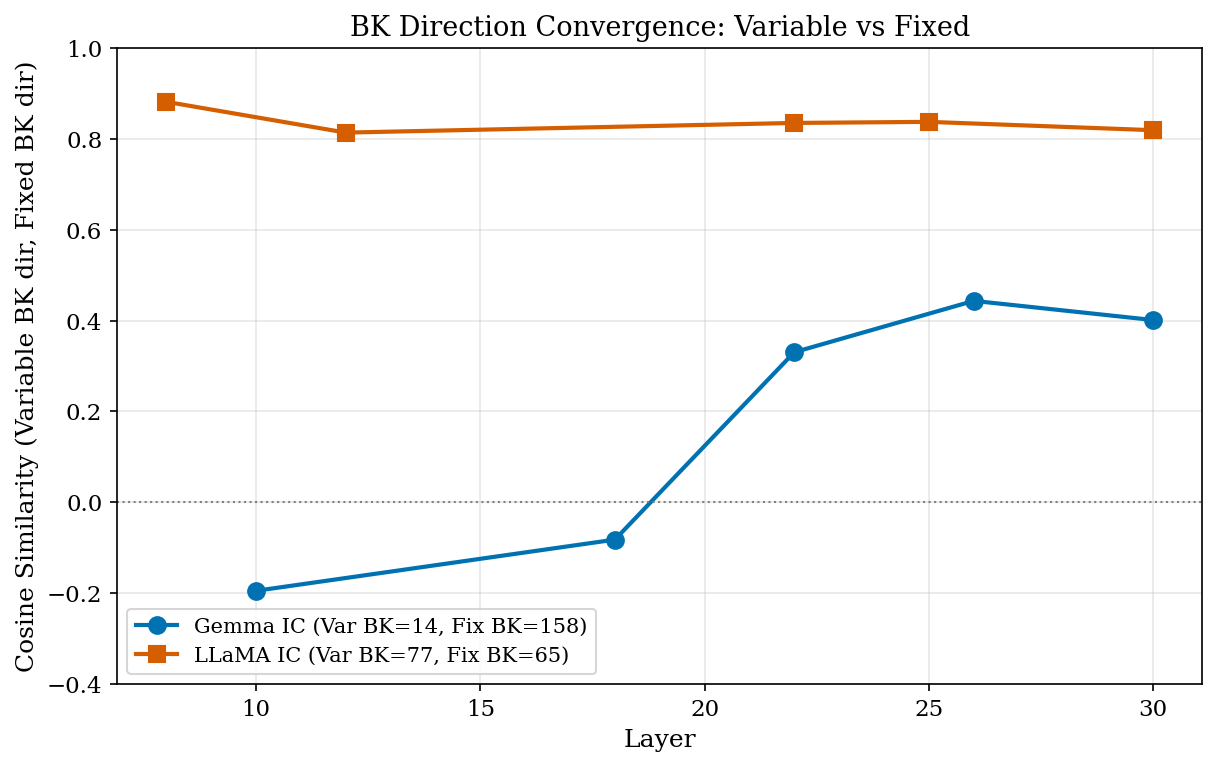
\includegraphics[width=\textwidth]{figures/fig2_bk_direction_crossmodel.png}
\caption{BK direction cosine across layers --- Gemma vs LLaMA IC. Gemma (blue): negative at shallow, positive at deep. LLaMA (orange): $\cos > 0.81$ at all layers. Gemma's shallow negative is likely a sample-size artifact (Var BK=14 vs LLaMA's balanced 77 vs 65).}
\label{fig:f5}
\end{figure}

\noindent\textbf{Caveat}: Gemma IC Variable BK=14 is extremely small. LLaMA's balanced sample (77 vs 65) provides more reliable estimates. When sample sizes are balanced, BK directions converge at all depths.

\subsection{Shared BK Neurons (Interaction Regression)}

Per-neuron regression: \texttt{activation $\sim$ $\beta_1$\textperiodcentered outcome + $\beta_2$\textperiodcentered bet\_type + $\beta_3$\textperiodcentered (outcome $\times$ bet\_type)}. Shared BK neurons: $\beta_1$ significant ($p<0.01$) + $\beta_3$ not significant --- BK effect is independent of bet-type.

\begin{table}[H]
\centering
\caption{Shared BK Neurons Across Models and Paradigms}\label{tab:t22}
\footnotesize
\begin{tabular}{lccc}
\toprule
 & Gemma IC L22 & LLaMA IC L22 & LLaMA SM L22 \\
\midrule
$n$\_neurons      & 3,584 & 4,096 & 4,096 \\
$n$\_BK           & 172   & 142   & 1,164 \\
Outcome-sig       & 1,639 (45.7\%) & 3,150 (76.9\%) & 1,052 (25.7\%) \\
Bet-type-sig      & 3,225 (90.0\%) & 3,742 (91.4\%) & 3,027 (73.9\%) \\
Interaction-sig   & 448 (12.5\%) & 1,605 (39.2\%) & 1,495 (36.5\%) \\
\textbf{Shared BK} & \textbf{1,182 (33.0\%)} & \textbf{1,501 (36.6\%)} & \textbf{72 (1.8\%)} \\
\bottomrule
\end{tabular}
\end{table}

\noindent Gemma IC 33.0\% and LLaMA IC 36.6\% --- similar proportions of bet-type-independent BK neurons across architectures. LLaMA SM shows only 1.8\% shared neurons because SM BK concentrates in Variable games (72.3\% vs 0.4\%), making ``bet-type-independent'' BK neurons nearly impossible.

\begin{figure}[H]
\centering
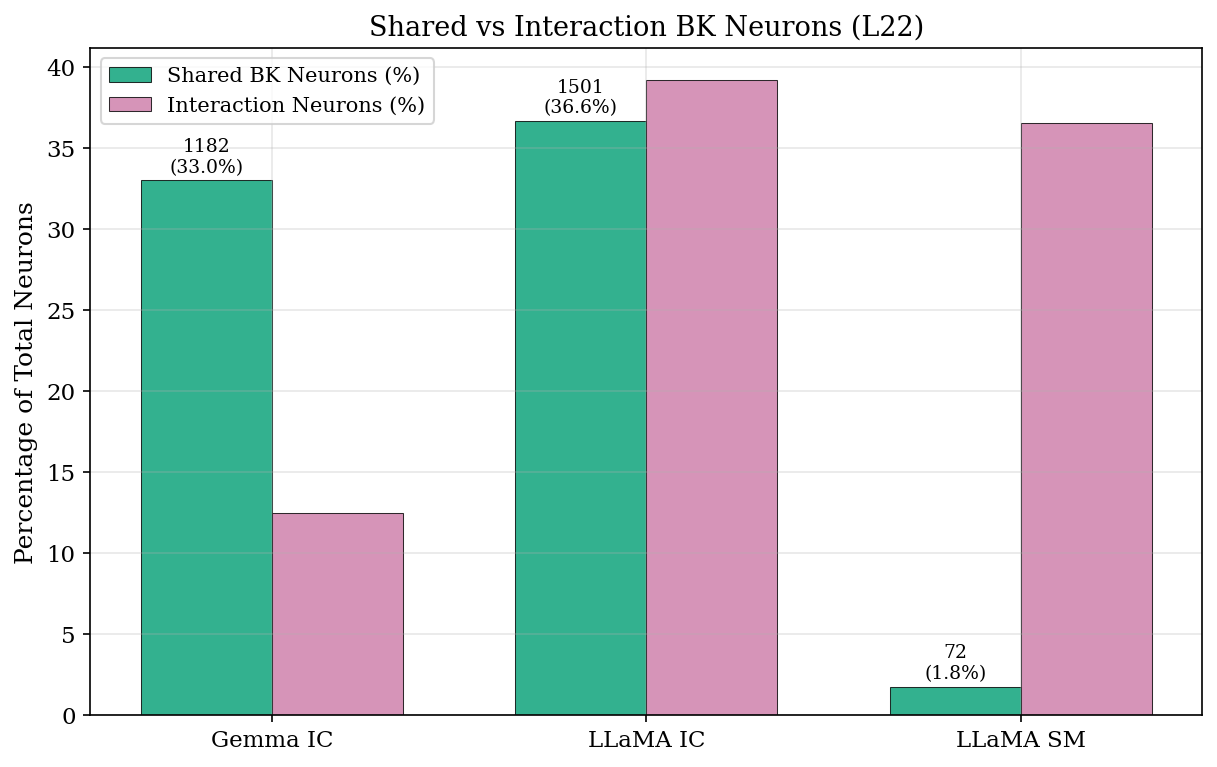
\includegraphics[width=\textwidth]{figures/fig7_shared_bk_neurons.png}
\caption{Shared vs Interaction BK neurons. Gemma IC (33.0\%) and LLaMA IC (36.6\%) show similar proportions. LLaMA SM (1.8\%) reflects Variable-dominated BK structure.}
\label{fig:f6}
\end{figure}

\subsection{Balance Confound Control}

\begin{table}[H]
\centering
\caption{Balance Partial Correlation (L22)}\label{tab:t23}
\footnotesize
\begin{tabular}{lcc}
\toprule
 & Gemma IC & LLaMA IC \\
\midrule
Raw BK-sig neurons       & 2,578 & 3,238 \\
Balance-controlled       & 2,569 & 3,269 \\
Retained                 & \textbf{99.7\%} & \textbf{101.0\%} \\
\bottomrule
\end{tabular}
\end{table}

\noindent Balance removal preserves 99.7--101\% of BK signal. BK representation encodes strategic/behavioral patterns, not simply balance information. LLaMA's 101\% indicates balance acts as a suppressor variable.

\subsection{Prompt Component Analysis (G/M/W/P/R)}

\textbf{Gemma SM} uses hidden state neurons (3,584-dim, 6 layers). \textbf{LLaMA SM} uses SAE features (32K, 5 layers). Direct absolute counts are not comparable; percentages are used.

\begin{table}[H]
\centering
\caption{Prompt Component BK Rate Effects (Cross-Model)}\label{tab:t24}
\footnotesize
\begin{tabular}{lccc}
\toprule
Component & Gemma SM ratio & LLaMA SM ratio & Cross-model \\
\midrule
\textbf{G} (Goal)   & \textbf{20.75$\times$} & 1.26$\times$ & Gemma $\gg$ LLaMA \\
M (Mood/Money) & 2.35$\times$  & 1.31$\times$ & Gemma $>$ LLaMA \\
W (Warning)    & 2.35$\times$  & 1.15$\times$ & Gemma $>$ LLaMA \\
H (Hint)       & ---           & 1.05$\times$ & LLaMA only \\
R (Reset)      & 1.72$\times$  & ---           & Gemma only \\
P (Persona)    & 1.17$\times$  & 1.06$\times$ & Both negligible \\
\bottomrule
\end{tabular}
\end{table}

\begin{table}[H]
\centering
\caption{Gemma SM Neural Analysis (comp $\times$ BK interaction neurons)}\label{tab:t25}
\footnotesize
\begin{tabular}{lccccccc}
\toprule
Comp. & L10 & L18 & L22 & L26 & L30 & L33 & Pattern \\
\midrule
G & 109 & 168 & 168 & 308 & \textbf{552} & \textbf{592} & Increases with depth \\
M & 41  & 23  & 25  & 10  & 8   & 15  & Negligible \\
R & 205 & 314 & 235 & 102 & 95  & 97  & Mid $\rightarrow$ decreasing \\
W & 183 & 70  & 23  & 1   & 0   & 0   & Vanishes with depth \\
P & 53  & 39  & 38  & 8   & 5   & 3   & Negligible \\
\bottomrule
\end{tabular}
\end{table}

\begin{table}[H]
\centering
\caption{BK-Amplifying Interaction Neurons (Gemma SM)}\label{tab:t26}
\footnotesize
\begin{tabular}{lcccl}
\toprule
Comp. & L10 & L22 & L30 & Interpretation \\
\midrule
G    & 0  & 0  & 1  & G drives BK independently; does not modulate BK \\
R    & 18 & 63 & 15 & R amplifies BK at mid-layers \\
W    & 42 & 3  & 0  & W has shallow-only BK amplification \\
M, P & 2--12 & 3--6 & 0 & Negligible \\
\bottomrule
\end{tabular}
\end{table}

\begin{table}[H]
\centering
\caption{LLaMA SM Neural Analysis (\% of active SAE features)}\label{tab:t27}
\footnotesize
\begin{tabular}{lccccl}
\toprule
Comp. & L8 int\% & L12 int\% & L30 int\% & L30 amp\% & Pattern \\
\midrule
G & 45.5\% & 61.5\% & \textbf{63.0\%} & 8.2\% & Interaction $\uparrow$ depth; low amp \\
M & \textbf{55.4\%} & 48.2\% & \textbf{51.2\%} & \textbf{14.5\%} & Highest amp all layers \\
H & 25.9\% & 31.2\% & 33.3\% & 7.4\% & Weak \\
W & 36.2\% & 37.2\% & 19.2\% & 5.8\% & Shallow-strong, deep-weak \\
P & 26.0\% & 27.1\% & 31.2\% & 4.8\% & Weak \\
\bottomrule
\end{tabular}
\end{table}

\begin{figure}[H]
\centering
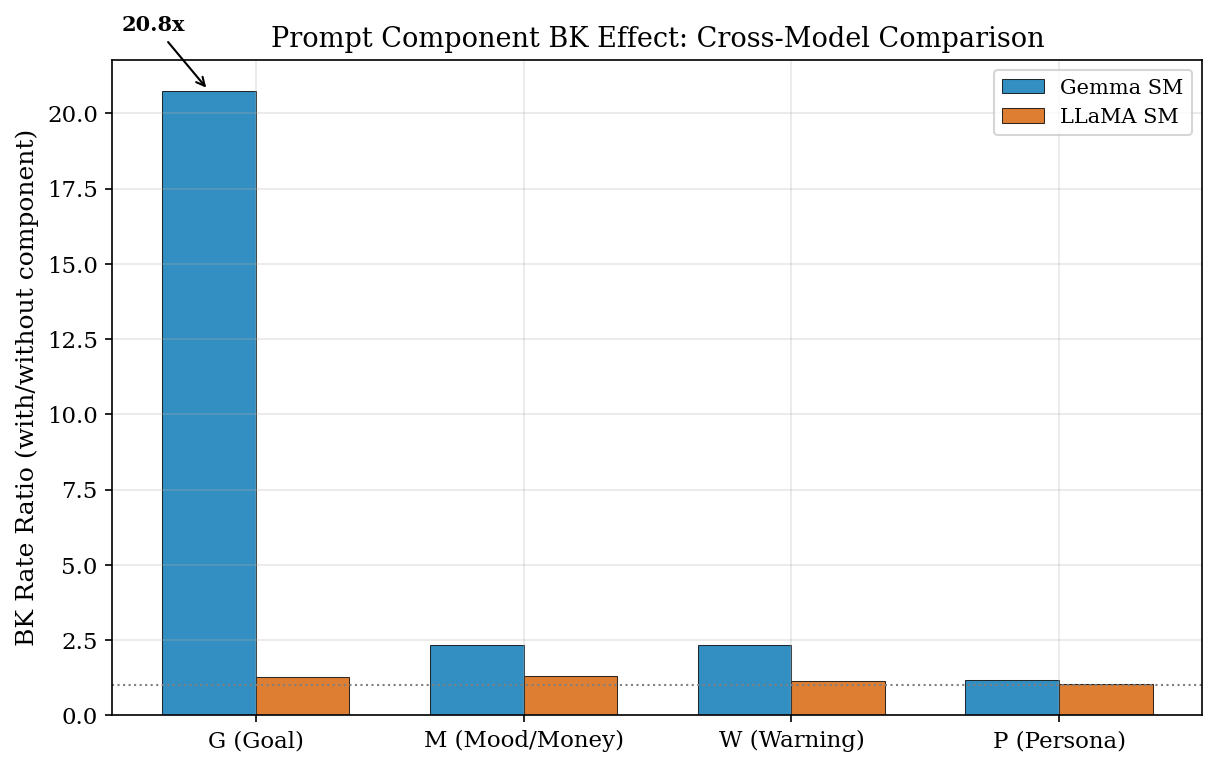
\includegraphics[width=\textwidth]{figures/fig5_prompt_components.png}
\caption{Prompt component BK effect. G(Goal) produces $20.8\times$ BK increase in Gemma (dominant) but only $1.26\times$ in LLaMA. Same prompt, $16\times$ different behavioral effect. M, W, P are weak in both.}
\label{fig:f7}
\end{figure}

\noindent G drives BK independently in both models (amplifies\_bk $\approx 0$ in Gemma, 8.2\% in LLaMA). Warning effects are shallow-only in both models (vanishes at deep layers). M(Money) is LLaMA's highest BK amplifier (14.5\% at L30), negligible in Gemma.

\subsection{G-Prompt BK Direction Alignment (Gemma L22)}

G-prompt direction ($\mathrm{G_{mean}} - \mathrm{nonG_{mean}}$) vs BK direction ($\mathrm{BK_{mean}} - \mathrm{Safe_{mean}}$) cosine:

\begin{table}[H]
\centering
\caption{G-Prompt Alignment}\label{tab:t28}
\footnotesize
\begin{tabular}{lccc}
\toprule
Paradigm & $\cos(G, BK)$ & BK with G & BK without G \\
\midrule
IC & $-$0.143 & 10.9\% & 10.6\% \\
SM & \textbf{+0.850} & 5.2\% & 0.3\% \\
MW & +0.367 & 2.5\% & 0.9\% \\
\bottomrule
\end{tabular}
\end{table}

\noindent In SM, G-prompt direction aligns strongly with BK direction ($\cos=+0.85$). G pushes the activation space directly toward BK. This is consistent with G driving BK independently --- G moves the hidden state toward BK without modulating existing BK representations.

\subsection{Bet Constraint Linear Mapping (Gemma IC L22)}

\begin{table}[H]
\centering
\caption{Bet Constraint $\rightarrow$ BK Projection}\label{tab:t29}
\footnotesize
\begin{tabular}{lccc}
\toprule
Constraint & $n$ & Mean BK prob & Actual BK rate \\
\midrule
c10 (\$1--\$10)  & 400 & 0.000 & 0.0\% \\
c30 (\$1--\$30)  & 400 & 0.056 & 5.2\% \\
c50 (\$1--\$50)  & 400 & 0.212 & 16.8\% \\
c70 (\$1--\$70)  & 400 & 0.270 & 21.0\% \\
\bottomrule
\end{tabular}
\end{table}

\noindent Linear correlation: $r=0.979$, $p=0.021$. (V8: $r=0.98$, nearly identical.)

\subsection{RQ3 Synthesis}

\begin{table}[H]
\centering
\caption*{\textbf{RQ3 Evidence Summary}}
\footnotesize
\begin{tabular}{lll}
\toprule
Evidence & Strength & Source \\
\midrule
LLaMA IC Var/Fix $\cos>0.81$ (all layers) & \textbf{Strong} & Balanced sample (77 vs 65), \S\ref{sec:bkdir} \\
Shared BK neurons $\sim$33--37\% (both IC) & \textbf{Strong} & Cross-model consistent \\
Balance confound control (both models) & \textbf{Strong} & 99.7--101\% retained \\
G independent BK driver (both models) & \textbf{Strong} & amp\_bk$\approx$0 (Gemma), 8.2\% (LLaMA) \\
W shallow pattern (both models) & \textbf{Moderate} & Vanishes deep in both \\
Gemma IC Var/Fix $\cos$ convergence & \textbf{Moderate} & Deep $\cos>0.33$ but Var BK=14 \\
G behavioral effect size difference & \textbf{Caution} & 20.75$\times$ vs 1.26$\times$ \\
M amplification difference & \textbf{Moderate} & LLaMA M=14.5\%, Gemma M$\approx$0 \\
\bottomrule
\end{tabular}
\end{table}

% ============================================================
% 5. LIMITATIONS
% ============================================================
\section{Limitations \& Critical Assessment}

\subsection{Permutation-Validated Claims}

\begin{table}[H]
\centering
\caption{Validated vs.\ Unvalidated Claims}\label{tab:validated}
\footnotesize
\begin{tabular}{lll}
\toprule
Claim & Test & Result \\
\midrule
Factor decomposition 67--71\% & 100-perm shuffle & $p=0.000$ (null 1\%) \checkmark \\
BK-inhibiting L30 & Binomial & All $p < 0.001$ \checkmark \\
Classification AUC & 100-perm shuffle & $p=0.000$ \checkmark \\
Gemma 3-par.\ consistency (L18+) & Binomial vs 25\% & $p < 5\times10^{-3}$ \checkmark \\
BK-inhibiting L22 & Binomial & LLaMA SM $p=0.897$ $\times$ \\
Variable cross-domain $d$\_corr & Bootstrap & mean=$-$0.075, CI incl.\ 0 $\times$ \\
\bottomrule
\end{tabular}
\end{table}

\subsection{Cross-Model Effect Size Confound}

\begin{table}[H]
\centering
\caption{Effect Size Confound}\label{tab:effsize}
\footnotesize
\begin{tabular}{lcc}
\toprule
 & Gemma SM & LLaMA SM \\
\midrule
$n$\_BK    & 87    & 1,164 \\
mean $|d|$ & 0.571 & 0.209 \\
\% $d\ge0.3$ & 68.8\% & 23.2\% \\
\bottomrule
\end{tabular}
\end{table}

\noindent Gemma's higher $|d|$ likely reflects small-sample inflation ($N=87$ $\rightarrow$ noisy, inflated estimates). LLaMA's lower $|d|$ may converge to true effects with larger $N$. \textbf{Cross-model effect size comparison is unreliable.} Classification AUC is a more robust comparison metric.

\subsection{Statistical Power Issues}

\begin{table}[H]
\centering
\caption{Statistical Power Limitations}\label{tab:power}
\footnotesize
\begin{tabular}{lll}
\toprule
Analysis & Weakness & Impact \\
\midrule
Var BK direction (Gemma IC) & $n_{\mathrm{var\_bk}}=14$ & Cosine: single estimate, unknown CI \\
LLaMA sign-consistency & Chance=50\%; 13/16 NS & Weak cross-domain evidence \\
Gemma L10, L12 & Binomial NS ($p>0.05$) & Shallow signal may be noise \\
\bottomrule
\end{tabular}
\end{table}

\subsection{Multiple Comparison Issues}

FDR correction is not systematically applied across all analyses. Expected false positives: Interaction regression (3,584 neurons $\times$ t-tests $\rightarrow$ $\sim$36 FP at $p<0.01$); Factor decomposition (581 features $\rightarrow$ $\sim$6 FP); Prompt analysis (3,584 $\times$ 5 components $\times$ 6 layers $\rightarrow$ many tests). Transfer analyses use permutation tests, partially addressing this. For other analyses, effect size (Cohen's $d$) should be treated as primary, $p$-values as secondary.

\subsection{Data Constraints}

\begin{enumerate}[nosep]
    \item \textbf{LLaMA MW not extracted}: 3-paradigm cross-model comparison not possible.
    \item \textbf{Gemma IC Variable BK=14}: Very limited power for bet-type comparisons.
    \item \textbf{MW Variable BK=4}: Below threshold ($n=5$), MW bet-type comparison not possible.
    \item \textbf{LLaMA hidden states}: Only 5 layers extracted (L8,12,22,25,30), not all 32.
    \item \textbf{No causal validation}: All analyses are correlational. Activation patching needed.
\end{enumerate}

\subsection{BK Rate Heterogeneity}

Gemma IC Fixed 19.75\% vs Variable 1.75\%; LLaMA IC Fixed 8.1\% vs Variable 9.6\% (reversed); Gemma SM 2.7\% vs LLaMA SM 36.4\% (13$\times$). Cross-model and cross-paradigm comparisons must account for base rate confounds.

\subsection{Prompt Component Model-Dependence}

G component: Gemma 20.75$\times$, LLaMA 1.26$\times$. ``Prompt condition invariance'' applies to neural structure (both models show G drives BK independently) but not to behavioral effect size.

% ============================================================
% 6. NEXT STEPS
% ============================================================
\section{Next Steps}

\begin{enumerate}[nosep]
    \item \sout{\textbf{LLaMA Hidden State Extraction}} $\rightarrow$ \textbf{Completed (v9.4)}. Symmetric analyses done.
    \item \textbf{Activation patching}: Causal validation of top cross-domain features.
    \item \textbf{LLaMA MW extraction}: Complete 3-paradigm comparison.
    \item \textbf{IC$\rightarrow$SM transfer mechanism}: Investigate layer-specific alignment.
    \item \textbf{FDR correction}: Apply to all per-feature/per-neuron tests.
    \item \textbf{G component deep dive}: Explain $20.75\times$ vs $1.26\times$ divergence.
    \item \textbf{BK rate confound control}: Balanced subsampling for IC-SM re-analysis.
\end{enumerate}

% ============================================================
% APPENDIX
% ============================================================
\appendix
\section{Supplementary Tables}

\subsection{Hidden State (600 neurons) vs SAE (744 features)}

\begin{table}[H]
\centering
\caption{Comparison of Analysis Levels}\label{tab:a1}
\footnotesize
\begin{tabular}{lccc}
\toprule
Level & Cross-domain consistent & FDR? & Binomial sig? \\
\midrule
Hidden state (3584-dim, L22) & 600 (16.7\%) & Yes ($p<0.01$) & --- \\
SAE features (131K, 7 layers) & 744 (total), L18+ sig & No FDR & L18+ $p<5\times10^{-3}$ \\
\bottomrule
\end{tabular}
\end{table}

\noindent Hidden state (16.7\% universal, FDR-corrected) and SAE (L18+ significant vs chance) consistently support cross-domain BK signal existence.

\subsection{Gemma SM Prompt Component Detail}

\begin{table}[H]
\centering
\caption{Gemma SM Prompt Component BK Rates}\label{tab:a2}
\footnotesize
\begin{tabular}{lccc}
\toprule
Component & BK with & BK without & Ratio \\
\midrule
\textbf{G} (Goal) & 5.2\% & 0.2\% & \textbf{20.75$\times$} \\
M (Mood)     & 3.8\% & 1.6\% & 2.35$\times$ \\
W (Warning)  & 3.8\% & 1.6\% & 2.35$\times$ \\
R (Reset)    & 3.4\% & 2.0\% & 1.72$\times$ \\
P (Persona)  & 2.9\% & 2.5\% & 1.17$\times$ \\
\bottomrule
\end{tabular}
\end{table}

\subsection{LLaMA IC$\rightarrow$SM Complete Transfer Profile}

L5=0.269($p$=1.0), L8=0.417($p$=1.0), L10=0.373($p$=1.0), L12=0.280($p$=1.0), L15=0.522($p$=0.02), L20=0.493($p$=0.795), \textbf{L25=0.783($p$=0.000)}, L30=0.418($p$=1.0).

\end{document}
